% !TeX root = skripta-konstitutivni-vztahy.tex
% !TeX lastmodified = 2018-12-04

\subsection{Podmínka plasticity Drucker-Prager}\label{sec:drucker-prager}
Představuje de facto rozšíření Misesovy podmínky na materiály s~různou mezí kluzu v~tahu a~tlaku.
Redukované napětí podle této podmínky je dáno rovnicí
\begin{equation}
	\sigma_\text{red}^\text{DP}
	= \frac{m-1}{2} \left(\sigma_\text{I} + \sigma_\text{II} + \sigma_\text{III}\right)
	+ \frac{m+1}{2} \sqrt{\frac{1}{2} \left[ (\sigma_\text{I}-\sigma_\text{II})^2 + (\sigma_\text{I}-\sigma_\text{III})^2 + (\sigma_\text{II}-\sigma_\text{II})^2 \right]}
\end{equation}
nebo
\begin{equation}
	\sigma_\text{red}^\text{DP}
	= \frac{m-1}{2} I_1 + \frac{m+1}{2} \sqrt{I_1^2 - 3 I_2}
\end{equation}
kde
\begin{equation*}
	m = \frac{R_e^\text{tlak}}{R_e^\text{tah}}
\end{equation*}
a~v~Haighově prostoru hlavních napětí představuje kužel s~osou v~normále oktaedrické roviny.
\begin{figure}[h]
	\centering
	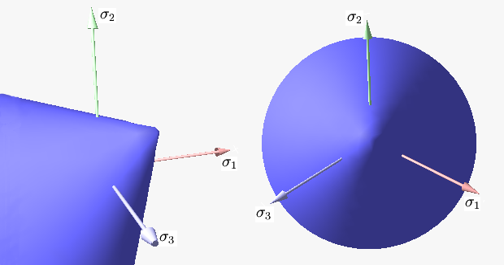
\includegraphics[width=0.5\linewidth]{drucker-prager}
	\caption{Podmínka plasticity Drucker-Prager v~Heighově prostoru}
	\label{fig:drucker-prager}
\end{figure}

Pozor! Pro výpočet součinitele bezpečnosti je třeba použít mez kluzu v~tlaku!
\begin{equation}
k = \frac{R_e^\text{tlak}}{\sigma_\text{red}^\text{DP}}
\end{equation}

Pro $m=1$ dostaneme standardní tvar Misesovy podmínky.
